% \documentclass{beamer}
% \usepackage{graphicx}
% \usepackage{multicol}
% \setlength{\columnseprule}{1pt}
%
% \graphicspath{{./fig/}}
% \usetheme{material}
% %%%%%%%%%%%%%%%%%%%%%%%%%%%%%%%%%%%%%%%%%%%%%%%%%%%%%%%%%%%%%%%%%%%%%%%%%%%%%%
% \embedvideo{<poster or text>}{<video file (MP4+H264)>}
% \embedvideo*{...}{...}                     % auto-play
%%%%%%%%%%%%%%%%%%%%%%%%%%%%%%%%%%%%%%%%%%%%%%%%%%%%%%%%%%%%%%%%%%%%%%%%%%%%%%

\ExplSyntaxOn
\NewDocumentCommand\embedvideo{smm}{
  \group_begin:
  \leavevmode
  \tl_if_exist:cTF{file_\file_mdfive_hash:n{#3}}{
    \tl_set_eq:Nc\video{file_\file_mdfive_hash:n{#3}}
  }{
    \IfFileExists{#3}{}{\GenericError{}{File~`#3'~not~found}{}{}}
    \pbs_pdfobj:nnn{}{fstream}{{}{#3}}
    \pbs_pdfobj:nnn{}{dict}{
      /Type/Filespec/F~(#3)/UF~(#3)
      /EF~<</F~\pbs_pdflastobj:>>
    }
    \tl_set:Nx\video{\pbs_pdflastobj:}
    \tl_gset_eq:cN{file_\file_mdfive_hash:n{#3}}\video
  }
  %
  \pbs_pdfobj:nnn{}{dict}{
    /Type/RichMediaInstance/Subtype/Video
    /Asset~\video
    /Params~<</FlashVars (
      source=#3&
      skin=SkinOverAllNoFullNoCaption.swf&
      skinAutoHide=true&
      skinBackgroundColor=0x5F5F5F&
      skinBackgroundAlpha=0
    )>>
  }
  %
  \pbs_pdfobj:nnn{}{dict}{
    /Type/RichMediaConfiguration/Subtype/Video
    /Instances~[\pbs_pdflastobj:]
  }
  %
  \pbs_pdfobj:nnn{}{dict}{
    /Type/RichMediaContent
    /Assets~<<
      /Names~[(#3)~\video]
    >>
    /Configurations~[\pbs_pdflastobj:]
  }
  \tl_set:Nx\rmcontent{\pbs_pdflastobj:}
  %
  \pbs_pdfobj:nnn{}{dict}{
    /Activation~<<
      /Condition/\IfBooleanTF{#1}{PV}{XA}
      /Presentation~<</Style/Embedded>>
    >>
    /Deactivation~<</Condition/PI>>
  }
  %
  \hbox_set:Nn\l_tmpa_box{#2}
  \tl_set:Nx\l_box_wd_tl{\dim_use:N\box_wd:N\l_tmpa_box}
  \tl_set:Nx\l_box_ht_tl{\dim_use:N\box_ht:N\l_tmpa_box}
  \tl_set:Nx\l_box_dp_tl{\dim_use:N\box_dp:N\l_tmpa_box}
  \pbs_pdfxform:nnnnn{1}{1}{}{}{\l_tmpa_box}
  %
  \pbs_pdfannot:nnnn{\l_box_wd_tl}{\l_box_ht_tl}{\l_box_dp_tl}{
    /Subtype/RichMedia
    /BS~<</W~0/S/S>>
    /Contents~(embedded~video~file:#3)
    /NM~(rma:#3)
    /AP~<</N~\pbs_pdflastxform:>>
    /RichMediaSettings~\pbs_pdflastobj:
    /RichMediaContent~\rmcontent
  }
  \phantom{#2}
  \group_end:
}
\ExplSyntaxOff
%
%% \newlength{\wdth}
%
%% \newcommand{\strike}[1]{\settowidth{\wdth}{#1}\rlap{\rule[.5ex]{\wdth}{.4pt}}#1}
%
%
%\begin{document}

% %%%%%%%%%%%%%%%%%%%%%%%%%%%%%%%%%%%%%%%%%%%%%%%%%%%%%%%%%%%%%%%%%%%%%%%%%%%%%%
% \embedvideo{<poster or text>}{<video file (MP4+H264)>}
% \embedvideo*{...}{...}                     % auto-play
%%%%%%%%%%%%%%%%%%%%%%%%%%%%%%%%%%%%%%%%%%%%%%%%%%%%%%%%%%%%%%%%%%%%%%%%%%%%%%

\ExplSyntaxOn
\NewDocumentCommand\embedvideo{smm}{
  \group_begin:
  \leavevmode
  \tl_if_exist:cTF{file_\file_mdfive_hash:n{#3}}{
    \tl_set_eq:Nc\video{file_\file_mdfive_hash:n{#3}}
  }{
    \IfFileExists{#3}{}{\GenericError{}{File~`#3'~not~found}{}{}}
    \pbs_pdfobj:nnn{}{fstream}{{}{#3}}
    \pbs_pdfobj:nnn{}{dict}{
      /Type/Filespec/F~(#3)/UF~(#3)
      /EF~<</F~\pbs_pdflastobj:>>
    }
    \tl_set:Nx\video{\pbs_pdflastobj:}
    \tl_gset_eq:cN{file_\file_mdfive_hash:n{#3}}\video
  }
  %
  \pbs_pdfobj:nnn{}{dict}{
    /Type/RichMediaInstance/Subtype/Video
    /Asset~\video
    /Params~<</FlashVars (
      source=#3&
      skin=SkinOverAllNoFullNoCaption.swf&
      skinAutoHide=true&
      skinBackgroundColor=0x5F5F5F&
      skinBackgroundAlpha=0
    )>>
  }
  %
  \pbs_pdfobj:nnn{}{dict}{
    /Type/RichMediaConfiguration/Subtype/Video
    /Instances~[\pbs_pdflastobj:]
  }
  %
  \pbs_pdfobj:nnn{}{dict}{
    /Type/RichMediaContent
    /Assets~<<
      /Names~[(#3)~\video]
    >>
    /Configurations~[\pbs_pdflastobj:]
  }
  \tl_set:Nx\rmcontent{\pbs_pdflastobj:}
  %
  \pbs_pdfobj:nnn{}{dict}{
    /Activation~<<
      /Condition/\IfBooleanTF{#1}{PV}{XA}
      /Presentation~<</Style/Embedded>>
    >>
    /Deactivation~<</Condition/PI>>
  }
  %
  \hbox_set:Nn\l_tmpa_box{#2}
  \tl_set:Nx\l_box_wd_tl{\dim_use:N\box_wd:N\l_tmpa_box}
  \tl_set:Nx\l_box_ht_tl{\dim_use:N\box_ht:N\l_tmpa_box}
  \tl_set:Nx\l_box_dp_tl{\dim_use:N\box_dp:N\l_tmpa_box}
  \pbs_pdfxform:nnnnn{1}{1}{}{}{\l_tmpa_box}
  %
  \pbs_pdfannot:nnnn{\l_box_wd_tl}{\l_box_ht_tl}{\l_box_dp_tl}{
    /Subtype/RichMedia
    /BS~<</W~0/S/S>>
    /Contents~(embedded~video~file:#3)
    /NM~(rma:#3)
    /AP~<</N~\pbs_pdflastxform:>>
    /RichMediaSettings~\pbs_pdflastobj:
    /RichMediaContent~\rmcontent
  }
  \phantom{#2}
  \group_end:
}
\ExplSyntaxOff

\section{Applications that might benefit from real-time}


\begin{frame}[label=app-110]
\frametitle{When the real-time flow information is crucial?}
\begin{itemize}
	\item Time-varying on slow time scales (e.g. sediment transport)
    \item Unpredictable start and duration (biology) 
    \item Irreproducible or expensive % add suction feeding stuff, ceramic particle release stuff, rupture and breakage
	\item Control of the flow-dependent process, or control the flow % add wind turbine stuff
    \item Mobility required, field experiments, harsh environments
\end{itemize}
\end{frame}

\begin{frame}[label=app-0]{Applications}
\centering\cardImg{lab1}{\textwidth}
\end{frame}

\begin{frame}[label=app-112]{We can leave the lab}
\begin{multicols}{2}
    \cardImg{ldc3}{.49\textwidth}
    \cardImg{ldc_splitter}{.49\textwidth}
\end{multicols}
\end{frame}


\begin{frame}[label=iibr-4]{And now we are ready for the Environmental Wind Tunnel}
    \cardImg{wind_tunnel_photo_1}{0.9\textwidth}
\end{frame}
    
\begin{frame}[label=iibr-44]{We are ready for the Environmental Wind Tunnel}
  \centering\cardImg{ptv_wind_tunnel_photo1.png}{.9\textwidth}
\end{frame}
    
\begin{frame}[label=app-22]{We can use it on a rotation table}
    \embedvideo{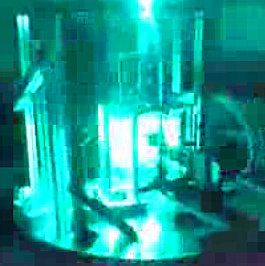
\includegraphics[width=\textwidth]{fig/rotation.jpg}}{video/rotation.mp4}
\end{frame}
    
    
    \begin{frame}[label=app-111]{Microgravity space applications}   
    \begin{columns}
    \column{.3\textwidth}
        \cardImg{microgravity}{\linewidth}
    \column{.7\textwidth}
        \cardImg{space_3d_ptv}{\linewidth}
    \end{columns}
    \end{frame}
    
    \begin{frame}[label=app-2]{Single camera with a four-view splitter}
    \centering\cardImg{kim/setup.png}{.95\textwidth}
    \end{frame}
    
    \begin{frame}[label=app-3]{Four view splitter}
    \embedvideo{
\includegraphics[width=\textwidth]{fig/kim/4views.png}}{fig/kim/Video1a.mp4}
    \end{frame}
    
    \begin{frame}[label=app-4]{Turbulent jet flow}
        \centering\cardImg{kim/jet.png}{\textwidth}
    \end{frame}

    


\begin{frame}[label=app-81]{Single camera - multiple views}
    \centering\cardImg{ldc_splitter}{0.8\textwidth}
    \embedvideo{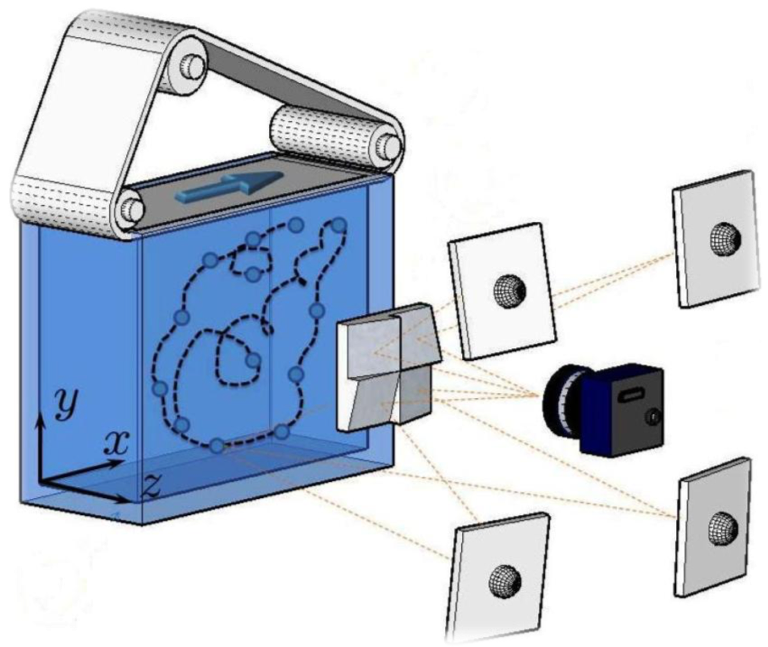
\includegraphics[width=\textwidth]{ldc_splitter}}{video/splitter_short.mp4}
    % \begin{cardTiny} A high speed camera with a four-view optical system \end{cardTiny}
    \end{frame}
    
    \begin{frame}[label=app-91]{3D-PTV can slide or rotate}
    \cardImg{sliding_ptv.jpg}{.9\textwidth}
    \begin{cardTiny} 
        Walpot et al. Meas. Sci. Tech. 2006. TU/e
    \end{cardTiny}
    \end{frame}
    
    
\begin{frame}[label=app-13]{3D-PTV main focus is turbulence}
    \begin{cardTiny} 
    Which means we need  the \alert{full gradient tensor} along the particle trajectories:
    $\partial u_{i}/\partial x_{j}$ in space and time
    \end{cardTiny}
    \begin{multicols}{2}
    \centering
    \cardImg{moffatt2}{.49\textwidth}
    \cardImg{ptvgif}{.49\textwidth}
    \end{multicols}
    \end{frame}
    
    \begin{frame}[label=app-14]{It had other applications, e.g. inertial clustering}
    \centering\cardImg{two_phase_3dptv}{.9\textwidth}
    \end{frame}
    
    \begin{frame}[label=app-15]{MRI + 3D-PTV}
    \begin{multicols}{2}
    \centering
    \cardImg{mri2}{.35\textwidth}
    \cardImg{mri3}{.35\textwidth}
    \end{multicols}
    \centering\cardImg{mri1}{.5\textwidth}
    \end{frame}
    
    
    \begin{frame}[label=iibr-2]
    \begin{multicols}{2}
    \centering
    \cardImg{camera_system_laser.jpg}{0.49\textwidth}
    \cardImg{calibration_in_laser.jpg}{.49\textwidth}
    \end{multicols}
    \begin{cardTiny}
    Four cameras point into the measurement location as seen from the test section inside the tunnel, and the calibration target is mounted on the traverse arm.
    \end{cardTiny}
    \end{frame}
    
    %
    \begin{frame}[label=iibr-1]
    \begin{multicols}{2}
    \centering\cardImg{img1.jpg}{.49\textwidth}
    \cardImg{camera_system_laser.jpg}{0.49\textwidth}
    \end{multicols}
    \end{frame}
    
    % \begin{frame}{Pressurized air seeding devices}
    % \cardImg{seeding_sources_2.jpg}{0.9\textwidth}
    % \end{frame}
    
    % \begin{frame}{Seeding material}
    % \centering\cardImg{SiO2_003}{0.75\textwidth}
    % \end{frame}
    
    
    % \subsection{3D Particle Tracking Velocimetry}
    
    %\begin{frame}
    %\centering\cardImg{volumes.png}{.6\textwidth}
    %\begin{cardTiny}
    %Representation in isometric view of the measurement sub-volumes within and above the canopy layer. The arrow points in the streamwise direction.
    %\end{cardTiny}
    %\end{frame}
    
    
    \begin{frame}[label=app-12]{Flow above the canopy}
    \centering
    \cardImg{flow_snapshot_above.jpg}{.9\textwidth}
    \end{frame}
    
    \begin{frame}[label=app-11]{Flow inside the canopy}
    \centering
    \cardImg{flow_snapshot_inside.jpg}{.9\textwidth}
    \end{frame}
    
    % \begin{frame}[label=app-10]{\href{./fig/flow_inside_laser.mp4}{Video clip}}
    % \centering\cardImg{flow_snapshot_inside.jpg}{\textwidth}
    % \end{frame}
    
%    
%    
    \begin{frame}[label=app-110]{You could also do PIV on FPGA}
    \cardImg{real_time_piv_fpga.png}{\textwidth}
    \begin{cardTiny}
    REAL-TIME PARTICLE IMAGE VELOCIMETRY
    BASED ON FPGA TECHNOLOGY, Munoz et al. IEEE (2009)
    \end{cardTiny}
    \end{frame}
%    
%    
    \begin{frame}[label=app-111]{Take it to the space}
    \cardImg{maser_8}{0.3\textwidth}
    \cardImg{space_3d_ptv}{0.6\textwidth}
    \begin{cardTiny}
    DESIGN AND CALIBRATION OF A FOUR-HEADED CAMERA SYSTEM
    FOR USE IN MICROGRAVITY RESEARCH, Willneff and Maas, 
    \end{cardTiny}
    \end{frame}
    

\begin{frame}[label=app-1]
    \frametitle{Suction feeding events, courtesy of Prof. Roi Holzman, TAU}
    \embedvideo{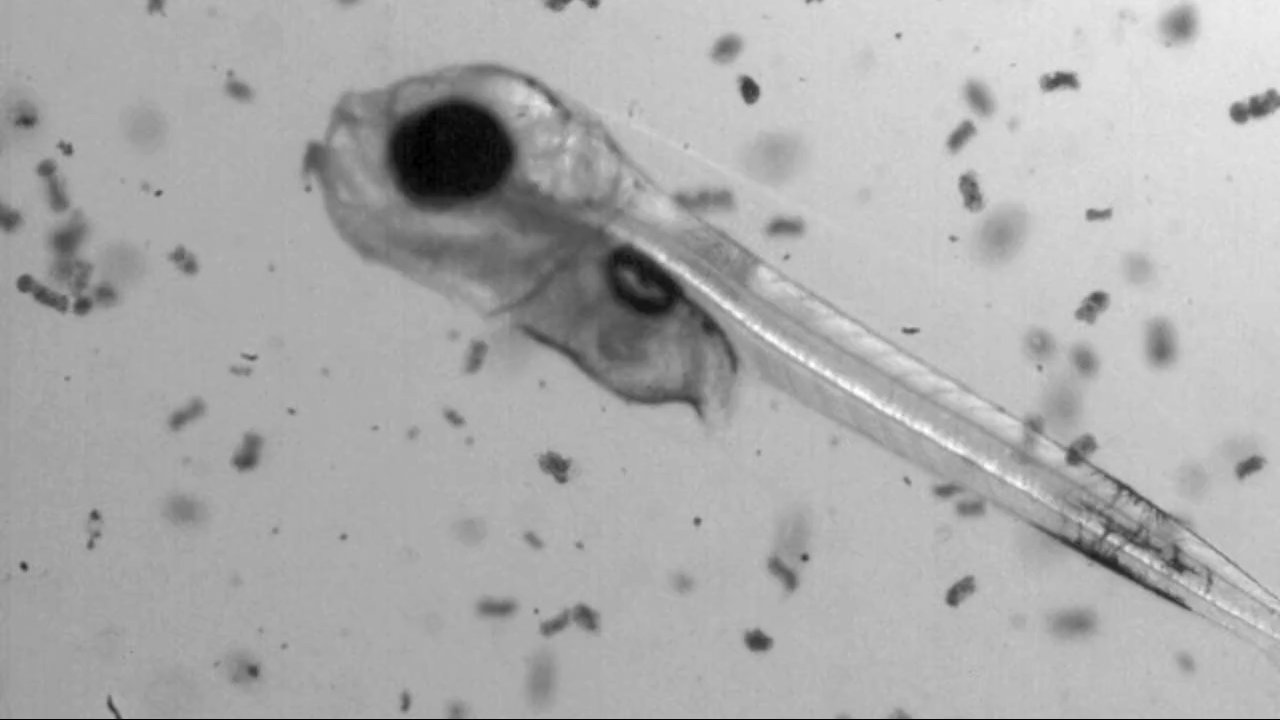
\includegraphics[width=\textwidth]{fig/fish_feeding.png}}{video/fish_feeding.mp4}
    %or this great video from Monterey Bay Aquarium 
    %
    %https://www.youtube.com/watch?v=umTqQSzKRmA    
\end{frame}
    
    \begin{frame}[label=app-2]
    \frametitle{Flamingo underwater feeding - San Diego Zoo}
    % https://www.youtube.com/watch?v=-1BF2XqboOo
    \begin{center}
    \embedvideo{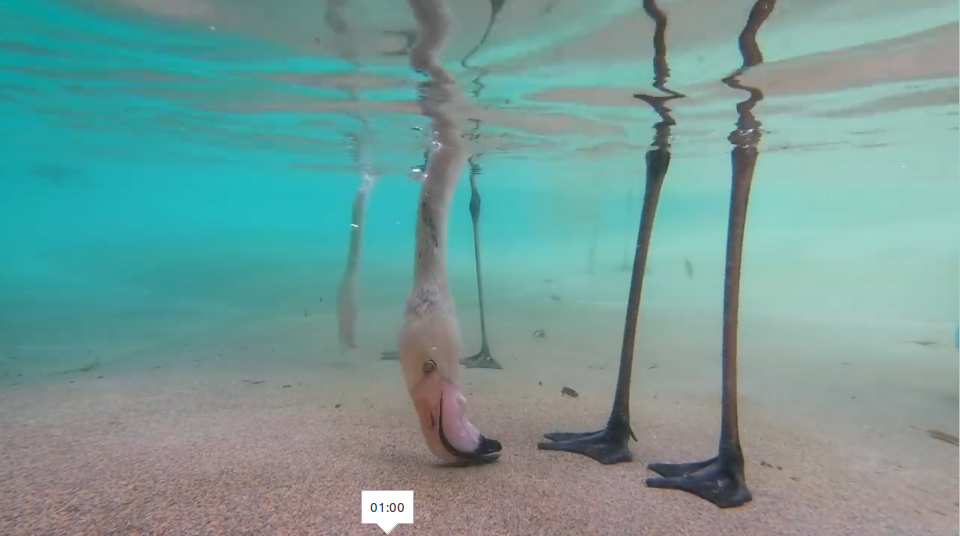
\includegraphics[width=\textwidth]{fig/flamingo.png}}{video/flamingo.mp4}
    \end{center}
    \end{frame}
    
    %
    
    \begin{frame}[label=app-31]
    \frametitle{Colloids breakage events in turbulent flow, ETH Zurich}
    %https://pubs.acs.org/doi/10.1021/acs.langmuir.5b03804
    \embedvideo{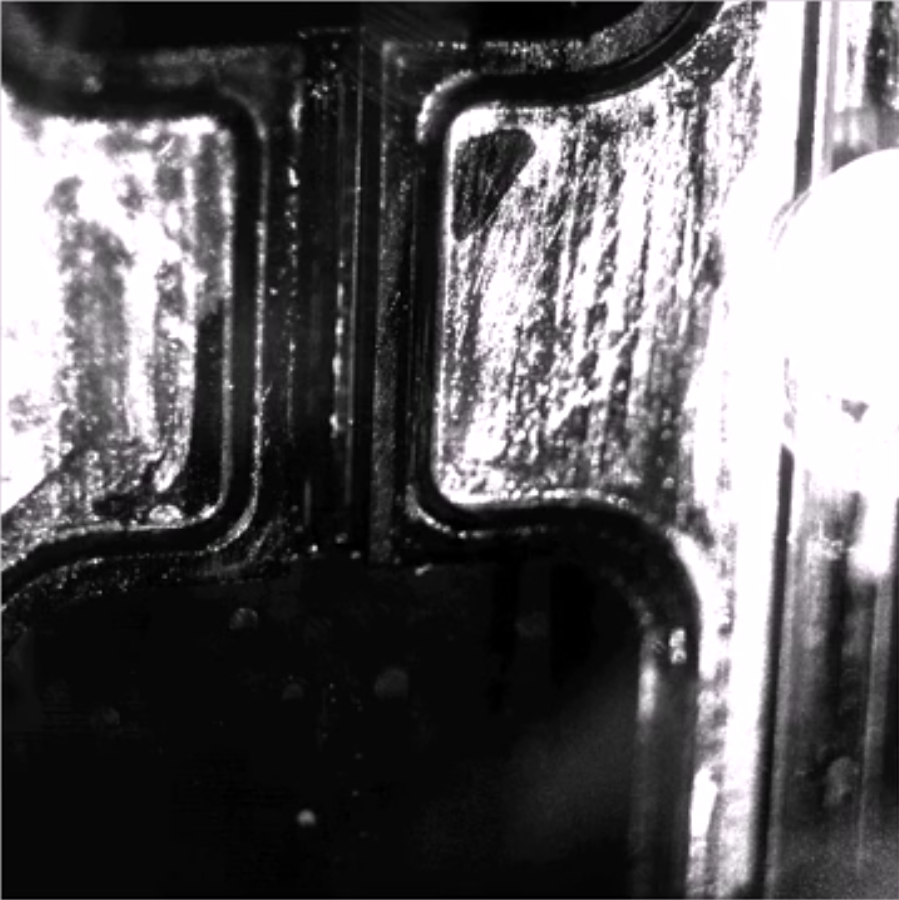
\includegraphics[width=\textwidth]{fig/colloids1.png}}{video/colloids1.mp4}
    \end{frame}
    
    %
    
    \begin{frame}[label=app-3]{Colloids breakage events in turbulent flow, ETH Zurich}
    %https://pubs.acs.org/doi/10.1021/acs.langmuir.5b03804
    \embedvideo{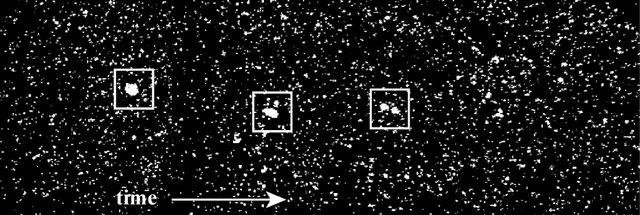
\includegraphics[width=\textwidth]{colloid_sequence.jpg}}{video/colloids2.mp4}
    \end{frame}
    
    
    
    \begin{frame}[label=app-4]{Aorta particle tracking velocimetry - rupture, ETH Zurich}
    \embedvideo{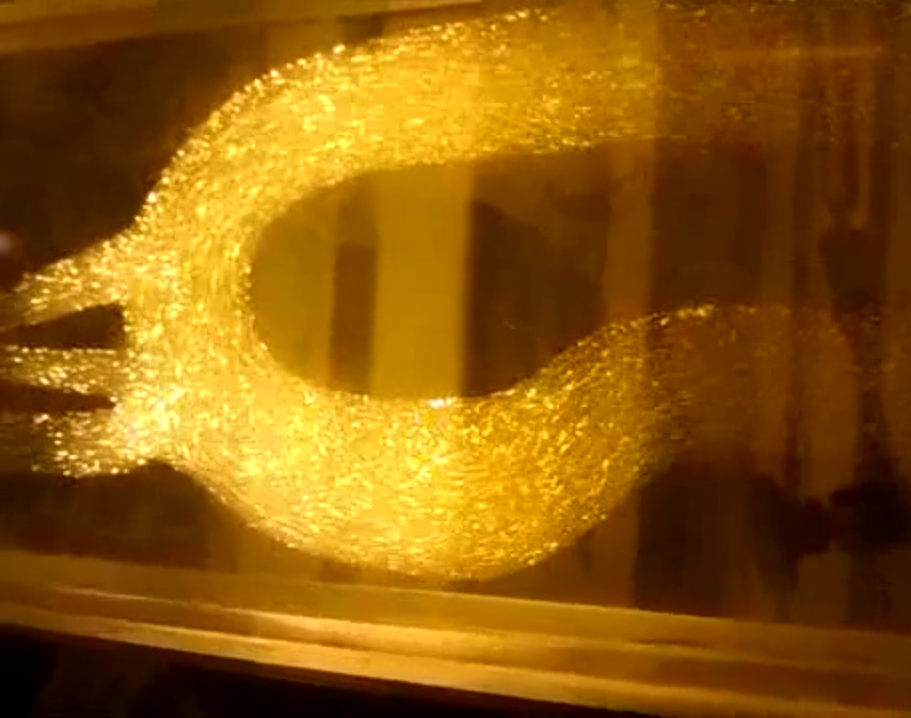
\includegraphics[width=\textwidth]{fig/aorta.png}}{video/aorta_rigid.mp4}
    \cardImg{aorta}{.9\textwidth}
    \end{frame}
    
    
    \begin{frame}[label=app-5]{Real time vortex identification for wind turbine blade pitch control - Caroline Braud}
    \begin{multicols*}{2}
    \cardImg{real_time_vortex_1}{.49\textwidth}
    \cardImg{real_time_vortex_2}{.49\textwidth}
    \end{multicols*}
    \end{frame}
    
    \begin{frame}[label=app-6]{Real-time sizing with 3D tracking - Rayne Ramirez, Uni. Oslo}
    \begin{multicols*}{2}
    \cardImg{drop-example}{.49\textwidth}
    \cardImg{drops}{.49\textwidth}
    \end{multicols*}
    \end{frame}
    
    \begin{frame}[label=app-7]{Fibers - Stefano Brizzolara, ETH Zurich}
    % https://twitter.com/stebrizzo94/status/1525577322144976910?s=20
    \embedvideo{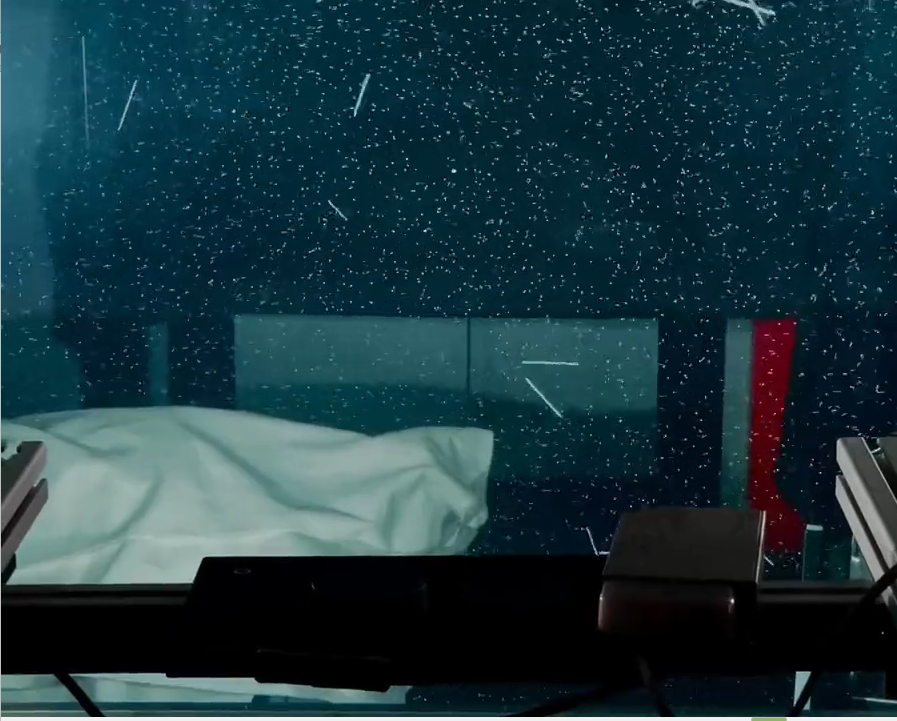
\includegraphics[height=\textheight]{fibers.png}}{video/fibers.mp4}
    
    \end{frame}
    
    \begin{frame}[label=app-8]{Drone vs turbulence - University of Minnesota}
    % Imaging‑based 3D particle tracking system forfield characterization ofparticle dynamics inatmospheric flows
    \embedvideo{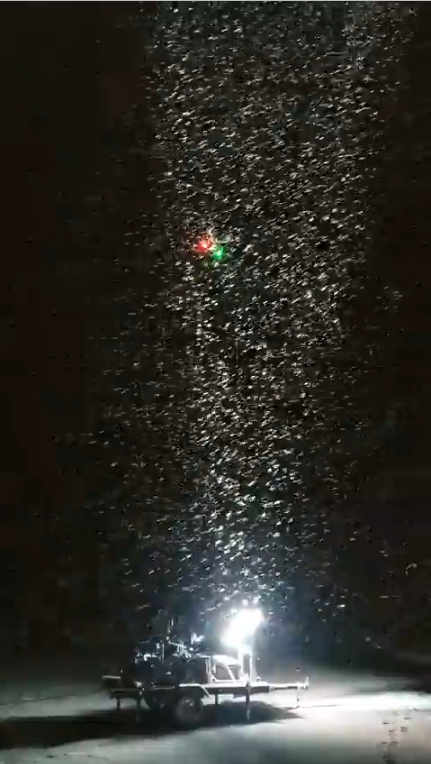
\includegraphics[height=\textheight]{drone.png}}{video/drone.mp4}\\
    Bristow et al. Exp. Fluids, 2023
    \end{frame}
    
    \begin{frame}[label=app-9]{Soon we could do it using AR/VR}
    \cardImg{mr_ptv_photo}{0.8\textwidth}
    Chivers, T. Uni. Vermont, MSc Thesis, 2023
    \end{frame}
    
    
    \begin{frame}[label=app-811]{Turbulent flow inside an urban canopy model - IIBR wind tunnel}
    \embedvideo{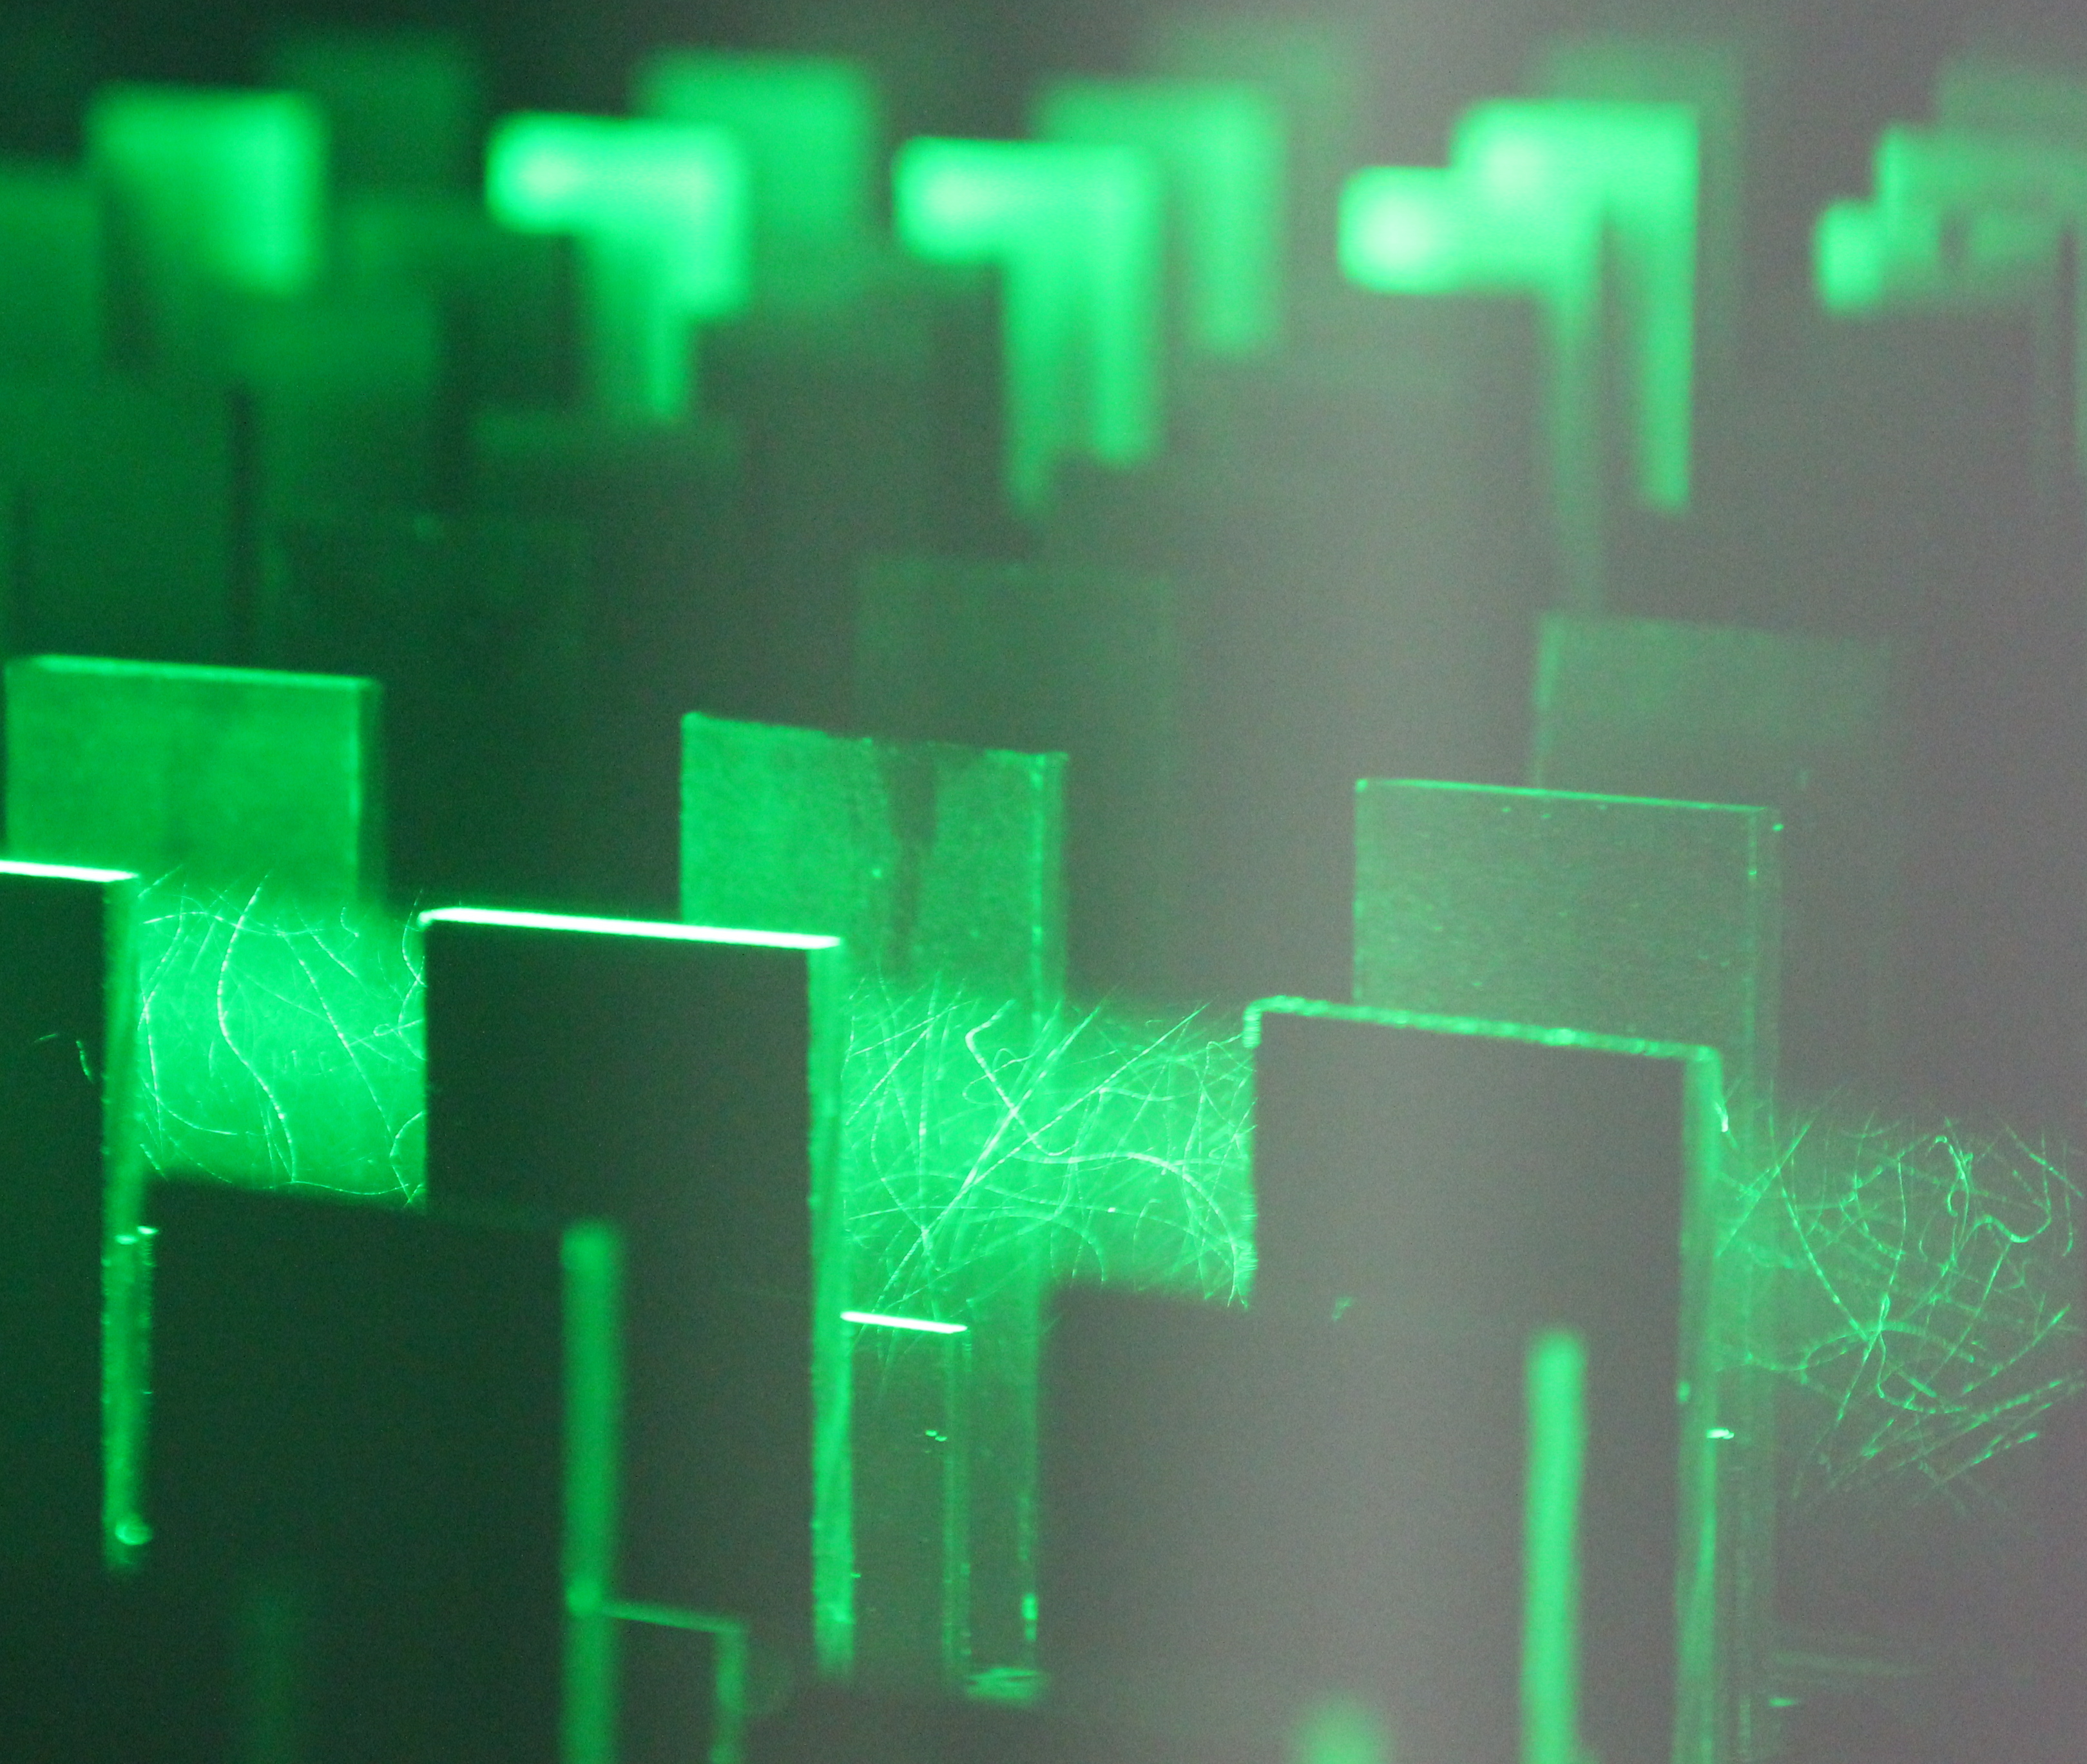
\includegraphics[width=\textwidth]{flow_snapshot_inside.jpg}}{video/flow_inside_laser.mp4}
    \end{frame}
%    

%\end{document}